\documentclass[utf8]{beamer}
\usetheme{Warsaw}

\usepackage[utf8]{inputenc}
\usepackage[english,russian]{babel}

\usepackage{url}
\usepackage{graphicx}
\usepackage{wrapfig}
\graphicspath{{img/}}

\title[Построение структурного выравнивания]{Построение и анализ структурного выравнивания молекул биополимеров в рамках проекта UGENE}
% Вариант: Инструменты построения и анализа СВ для UGENE
% Кстати, зоепиливать в тему "UniPro UGENE" или нет?
\author[Кузнецов Алексей]{Кузнецов Алексей гр. 7312 \linebreak научный руководитель Фурсов М.Ю. UniPro}
% Блин, куда научрука-то вкатить?
\institute{Новосибирский Государственный Университет}
\date{\today}

\begin{document}
% Итак, приступим...

\begin{frame}
\titlepage
\end{frame}

% Структурное выравнивание, что это такое
% Это попытка определить гомологичность двух белков
% на основе их третичной структуры
% Термин выравнивание взят по аналогии с выравниванием последовательностей
\begin{frame}{Структурное выравнивание}
\begin{columns}[c]
\column{0.5\linewidth}
	\center{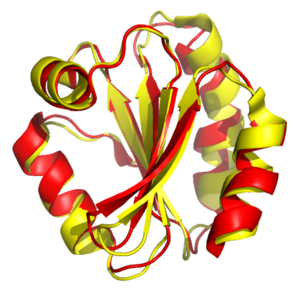
\includegraphics[width=\linewidth]{wiki.png}}
\column{0.5\linewidth}
	Определение гомологичности молекул биополимеров
	\begin{itemize}
		\item Белков
		\item РНК
	\end{itemize}
	по их третичной структуре

\end{columns}


\end{frame}

% Это важный инструмент структурной биологии
% Определение функционального назначения на основе структуры
% Сравнение белков с сильноразличающейся первичной структурой(аминокислотной последовательностью)
% Оценка алгоритмов предсказания структуры
\begin{frame}{В биологии}
\begin{itemize}
	\item Определение функционального назначения белка на основе структуры
	\item Сравнение белков с сильноразличающейся аминокислотной последовательностью
	\item Тестирование алгоритмов предсказания структуры
\end{itemize}
\end{frame}

% Входные данные это третичная структура, попросту 3х-мерная модель
% может усугубляться всякими дополнительными данными
% Источники экспериментальные NMR, X-Ray; смоделированные
% обычно записывается в файлы формата PDB
% Результат rmsd и матрица пребразования
\begin{frame}{Данные и результаты}
Данные
\begin{itemize}
	\item трехмерная модель
	\item дополнительные (например карта зарядов)
\end{itemize}
Источники
\begin{itemize}
	\item Измерение - NMR, X-Ray
	\item Моделирование - алгоритмы предсказания
\end{itemize}	
Формат - файлы PDB (\url{http://www.pdb.org})

\vspace{11pt}

Результаты
\begin{itemize}
	\item RMSD - root mean square deviation
	\item Матрица преобразований модели - сдвиг, поворот
\end{itemize}	
Можно экспортировать в PDB
\end{frame}

% Геометрический подход: выравниваем 2(попарное) или несколько(множественное) молекул
% минимизируя rmsd, визуализация получается довольно наглядная
% стул vs табуретка
\begin{frame}{Геометрический подход}
\begin{figure}[h]
\center{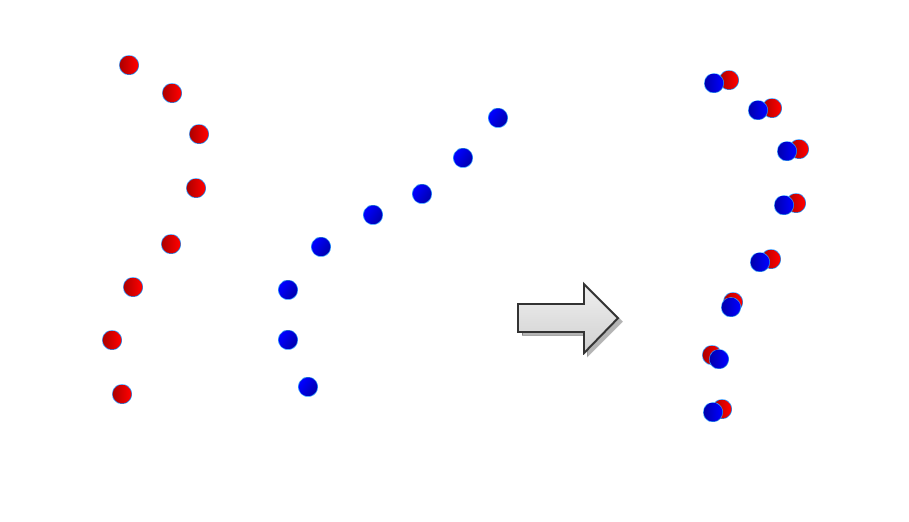
\includegraphics[width=\linewidth]{geom.png}}
\end{figure}
Поиск трансформации для наилучшего выравнивания
\end{frame}

% Слайд с кучей алгоритмов, немногие из них существуют в виде законченных продуктов
\begin{frame}{Существующие алгоритмы}
\begin{center}
\begin{small}
MAMMOTH CE/CE-MC DaliLite VAST PrISM SSAP SARF2 KENOBI/K2 STAMP MASS SCALI DEJAVU SSM SHEBA LGA POSA PyMOL FATCAT Matras MAMMOTH-mult Protein3Dfit PRIDE FAST C-BOP ProFit TOPOFIT MUSTANG URMS LOCK LOCK 2 CBA TetraDA STRAP LOVOALIGN GANGSTA GANGSTA+ TM-align MatAlign Vorolign EXPRESSO CAALIGN YAKUSA BLOMAPS CLEPAPS TALI F MolCom MALECON FlexProt MultiProt CTSS CURVE Matt TopMatch SSGS Matchprot UCSF Chimera  FLASH RAPIDO ComSubstruct ProCKSI SARST Fr-TM-align TOPS+ COMPARISON TOPS++ FATCAT MolLoc FASE SABERTOOTH STON SALIGN MAX-PAIRS THESEUS TABLEAUSearch QP Tableau Search ProSMoS MISTRAL MSVNS for MaxCMO Structal ProBiS ALADYN SWAPSC SA Tableau Search
\end{small}
\end{center}
\end{frame}

% Цель: реализовать такой инструмент в продукте UniPro UGENE
% Задачи: построение, визуализация, импорт/экспорт, оформление, основа для дальнейшего развития
\begin{frame}{Цель работы}
\begin{center}
\Large Реализовать инструменты построения и анализа структурных выравниваний для проекта UGENE
\end{center}
\vspace{11pt}
Задачи
\begin{itemize}
	\item Интеграция существующего алгоритма выравнивания
	\item Интерактивная визуализация результатов выравнивания
	\item Оформление алгоритма в виде вычислительной задачи UGENE
	\item Выделение API для дальнейшего развития
\end{itemize}
\end{frame}

% Пара слов о UGENE. Объединяет множество инструментов в одном формате.
% Уже имеет инструменты выравнивания последовательностей, визуализации макромолекул, ограниченную поддержку PDB
\begin{frame}{UGENE}
\begin{center}
\Large UniPro UGENE -- это открытое ПО для работы молекулярного биолога 
\end{center}
\begin{itemize}
	\item Десятки различных инструментов в единой модели данных
	\item Удобный графический интерфейс
	\item Инструменты выравнивания последовательностей
	\item Базовые инструменты визуализации макромолекул
	\item Частичная(ro) поддержка PDB и MMDB форматов
	\item Free as a speech and free as a beer
\end{itemize}
\end{frame}

% Слайд с картинками про UGENE
% Опенсорц free as a speech and free as a beer. Активно развивается.
\begin{frame}{UGENE}
\begin{figure}[h]
\center{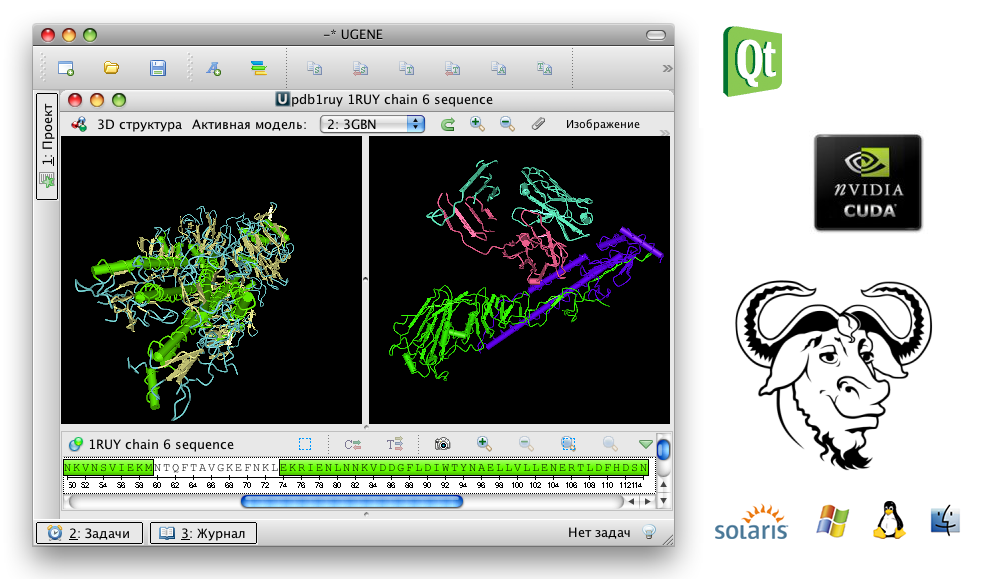
\includegraphics[width=\linewidth]{all.png}}
\end{figure}
\end{frame}

% Надо таки слайд с результатами
\begin{frame}{Прогресс}
\begin{itemize}
	\item Обзор существуэщих решений, как пакетов так и алгоритмов 
	\item Интегрирована библиотека ptools, идет её тестирование
	\item Идет работа над визуализацией
\end{itemize}
\end{frame}

% Спасибо за внимание
\begin{frame}{Q\&A}
\begin{center} 
Спасибо за внимание!
\end{center}
\end{frame}

\end{document}
